\section{Introduction}
\label{industry_needs}
As we mentioned in chapter \ref{chapter_general_intro}, the aim of this thesis has been twofold: deriving a methodology for inferring the motivational state of individuals while interacting with potentially rewarding object (a videogame in this case) and presenting how this could be used in an applied setting.

In this view, this chapter will focus on sketching the design of a system relying on our methodology for automated engagement prediction. First we will introduce a set of ethical considerations that should be taken into account when designing such system. Subsequently, we will provide an overview on why an industry player (or groups thereof) might need a process for quantifying and predicting engagement and which characteristics this process should have. Finally we will proceed at illustrating a system designed for serving this need, placing particular emphasis on how its components connect with the work presented so far.

\section{Some Ethical Consideration}
\label{ehtical_considerations}
Automated system leveraging behavioural data are now-days used extensively in both low and high stakes scenarios \cite{mehrabi2021survey}, with the potential to have a direct and concrete impact on individuals. For this reason, when designing automated data-driven applications, issues related to fairness should be taken into account. 

By fairness we entail the set of principles and considerations that in recent years are adopted in order to avoid that decisions based on a machine-learned model do not inadvertently bring harm to specific groups of people \cite{mehrabi2021survey}. A complete overview of the issue of fairness in machine learning would be beyond the scope of not just this section but the entire thesis, as it is a vast landscape \cite{mehrabi2021survey} hard to navigate due to its many levels of complexity \cite{corbett2018measure}.  We will therefore focus on two major aspects related to the work presented in this chapter. 

The first aspect concerns biases present in the data on which a machine learning algorithm is fitted. These might be induced by an over or under representation of certain strata of the population that an automated system will ultimately need to serve \cite{mehrabi2021survey}. Given how a large part of machine learning algorithms are fitted to the data (e.g., maximum likelyhood) the risk is that the prediction produced by the algorithm will revert to the mean or in the worst case, will result to be biased with respect to the true characteristics of the population \cite{corbett2018measure, mehrabi2021survey}. Despite the harm that these biases might cause in the context of engagement prediction is not as pronounced as in other areas (e.g., credit, criminal or medical risk assessment), they can still have unexpected repercussion on an individual. 

To this connects the second aspect of fairness that we want to highlight, namely the risk of inadvertently cause harm to individuals which are either temporarily or structurally subject to some form of vulnerability. This might happen as a consequence of automated decision making based on what we call "unconstrained model predictions"


for example if we imagine a system aimed at target high spender users in a game based on gatcha or loot-box mechanics, an unconstrained prediction might inadvertently target individual with a predisposition to or an history of problematic gambling behaviour.

\section{Engagement Quantification and Prediction for the Videogames Industry}
\label{industry_needs}
As we mentioned before despite the industry might be interested in the development of research projects the the focus of this project is less on the advancement of the research field on more focused on the solution of practical problems. 

In this view how does engagement connects with practical problems that the industry has? Very often (if not always) the success of a videogame title is strictly connected with either its ability to retain users or with the experience that users had with the product. The first is pivotal in scenarios where game is treated as a service sold to an audience (similarly to the function of streaming services) while the second is more relevant in scenarios where games are considered digital goods. 

In this context, engagement can be viewed as a measure of how a particular game was, is or will be able to retain users: if an individual is engaged with a particular service it is likely that will keep take advantage of it similarly if an individual had a particular good experience and gladly engaged with a particular digital good it is is more likely that will either suggest it to other users, buy similar products or buy product from the same seller.  

In this view being able to estimate the current propensity of a user towards a specific game translates (in a more or less direct way) to the capacity of assessing if a game is likely to be a success of public and revenue. For this reason it is often the case that videogame publishers and studios try to leverage the information they have available through telemetry system for taking the stock of how a particular game is performing. This is the classical example of analytical reports summarizing various type of game related Key Performance Indicators. 

\section{Multi-context Automated Engagement Prediction and Quantification}
\label{industry_needs}

\section{Data Generation}
\lorem
\subsection{Users}
\lorem
\subsection{Game Contexts}
\lorem

\section{Model Owner}
\lorem
\subsection{Data Storage}
\lorem
\subsection{Model Generation}
\lorem
\paragraph*{Data Generators} \lorem
\paragraph*{Model Configurations} \lorem
\paragraph*{Model Tuning} \lorem
\paragraph*{Model Training} \lorem
\paragraph*{Model Validation} \lorem
\paragraph*{Model Serving} \lorem

\section{Model Consumer}
\lorem
\subsection{Representation Sharing}
\lorem
\subsection{Profile Generation}
\lorem
\subsection{Live Predictions}
\lorem
\subsection{Automated Reporting}
\lorem

\begin{figure}[ht]
\centering
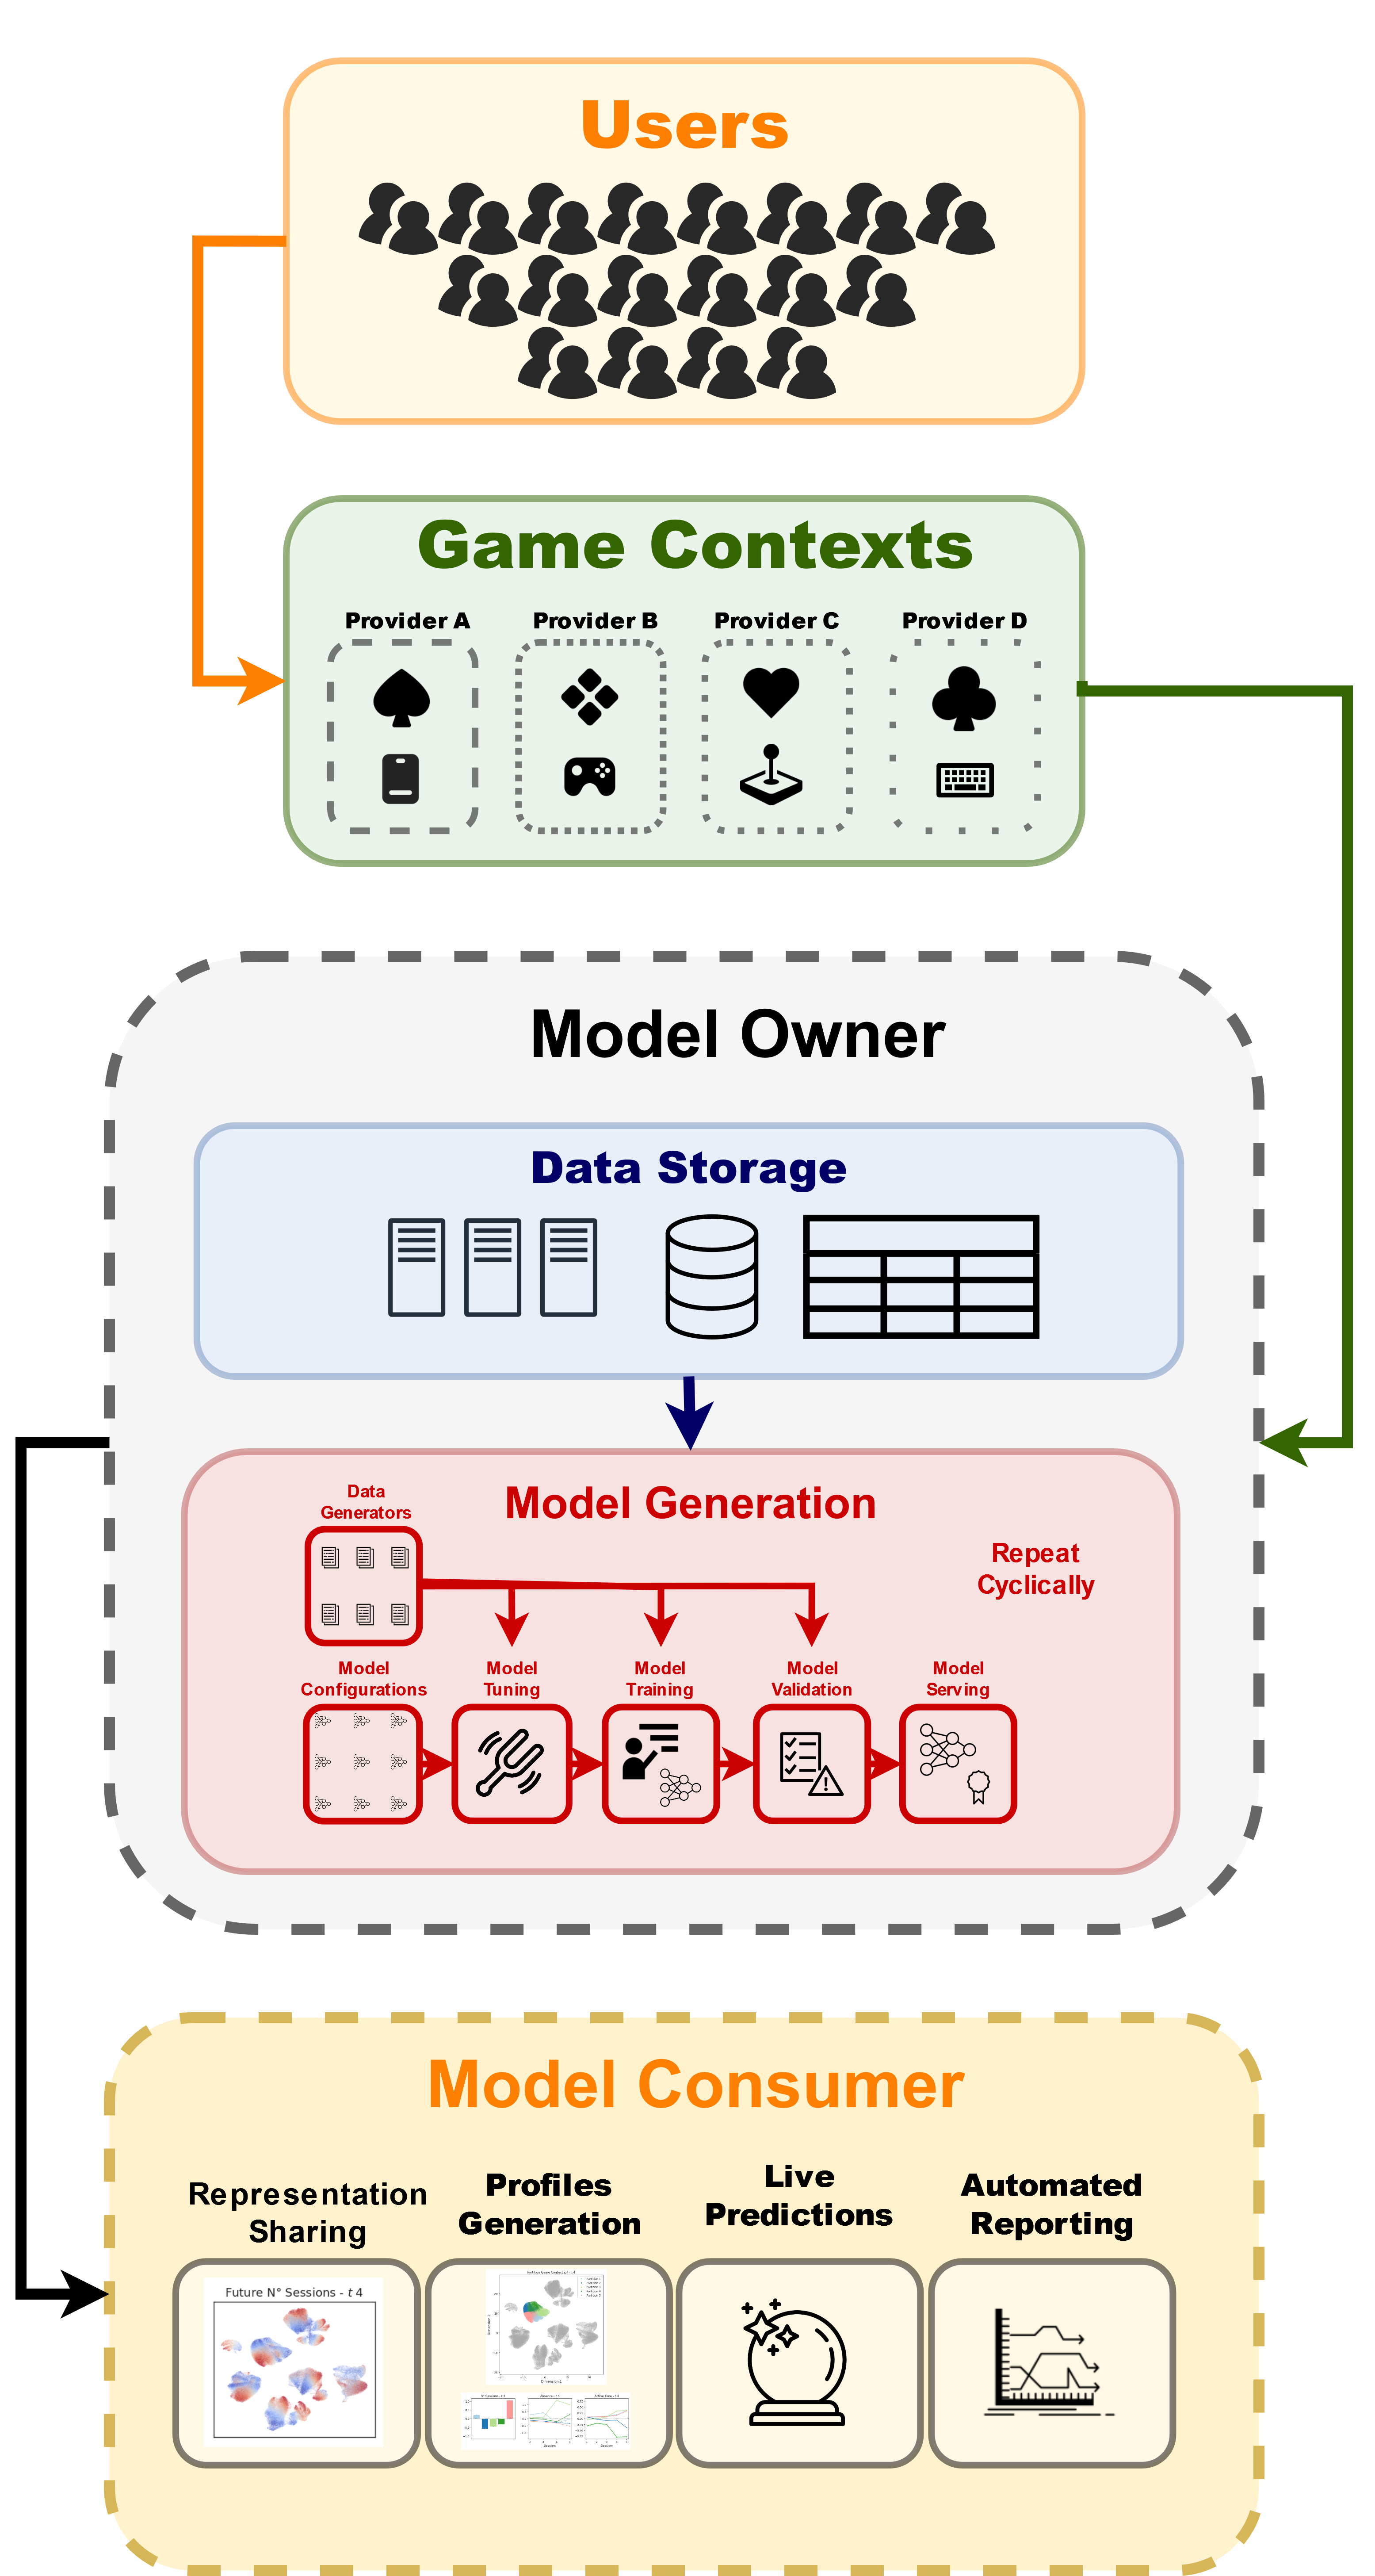
\includegraphics[width=0.7\textwidth]{images/chapter_5/pipeline_diagram.png}
\caption[\textbf{Model Deployment Pipeline}]{The figure represents a simplified system diagram for a potential application of the improved RNN architecture. Solid lines represent low-level components in the system while dashed lines indicate high-level entities. Directional arrows represent the flow of operations inside the system.}
\label{pipeline}
\end{figure}